\section{Potenzfunktionen}
\subsection{Einführung}
Sie kennen bereits folgende Typen von Funktionen:
\begin{itemize}
    \item lineare Funktionen: $f(x) = mx + q$
    \item quadratische Funktionen: $f(x)=ax^2+bx+c$
\end{itemize}
Wir werden nun eine weitere Klasse von Funktionen kennenlernen, die \textbf{Potenzfunktionen}.
\begin{deff}[Potenzfunktionen]{}
    Eine \textbf{Potenzfunktion} ist eine Funktion der Form $f(x) = x^n$, wobei $n\in \mathbb{Z}^*$ eine ganze Zahl ist.
\end{deff}
Im folgenden werden Sie selbstständig die wichtigsten Eigenschaften der Graphen der Potenzfunktionen untersuchen.
\subsubsection{Einführungsaufgabe}
\begin{enumerate}
    \item Füllen Sie die Tabelle auf der Rückseite wie folgt aus:
          \begin{enumerate}
              \item Die erste Spalte ist schon ausgefüllt und soll als Beispiel dienen.
              \item Gehen Sie Spalte für Spalte vor.
              \item Zeichnen Sie die Graphen der im Koordinatensystem angegebenen Funktionen in Geogebra und übertragen Sie die Skizze ins Koordinatensystem.
              \item Füllen Sie dann die Zellen von oben nach unten aus, indem Sie den Graphen untersuchen und sich überlegen, wie man die Erkenntnisse auch aus der Funktionsgleichung gewinnen könnte.
          \end{enumerate}
    \item Die Graphen mit negativem Exponenten verhalten sich rund um die Stelle $x=0$ besonders. Erklären Sie, wieso und auch welchen Einfluss es hat, wenn der Exponent gerade oder ungerade ist.
\end{enumerate}
\begin{landscape}

    \renewcommand{\arraystretch}{1.7}

    \begin{tabular}{|m{5cm}|m{4.5cm}|m{4.5cm}|m{4.5cm}|m{4.5cm}|}
        \hline
        $f(x) = x^n$                          & $n$ positiv und gerade                                                                                                       & $n$ positiv und ungerade                                               & $n$ negativ und gerade                                                 & $n$ negativ und ungerade \\
        \hline
        Graph

        (der im Bild vorgegebenen Funktionen) & 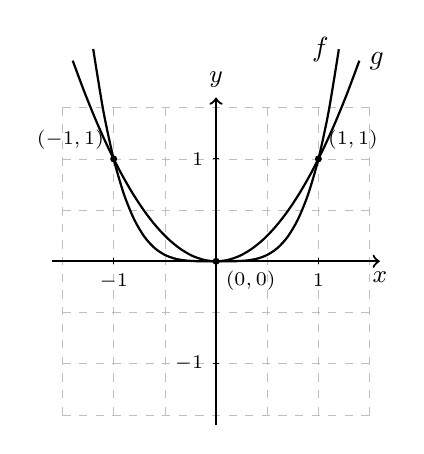
\begin{tikzpicture}[scale=1.3]
                                                    % Hintergrund-Gitter
                                                    \draw[step=0.5cm,gray!50,very thin,dashed] (-1.5,-1.5) grid (1.5,1.5);

                                                    % Achsen
                                                    \draw[->,thick] (-1.6,0) -- (1.6,0) node[below] {\small $x$};
                                                    \draw[->,thick] (0,-1.6) -- (0,1.6) node[above] {\small $y$};

                                                    % Funktionen
                                                    \draw[domain=-1.4:1.4,smooth,variable=\x,thick] plot ({\x},{\x*\x}) node[right] {$g$}; % g(x) = x^2
                                                    \draw[domain=-1.2:1.2,smooth,variable=\x,thick] plot ({\x},{\x*\x*\x*\x}) node[left] {$f$}; % f(x) = x^4

                                                    % Punkte einzeichnen
                                                    \filldraw (0,0) circle (0.8pt) node[below right] {\scriptsize $(0,0)$};
                                                    \filldraw (1,1) circle (0.8pt) node[above right] {\scriptsize $(1,1)$};
                                                    \filldraw (-1,1) circle (0.8pt) node[above left] {\scriptsize $(-1,1)$};

                                                    % Achsenbeschriftungen
                                                    \foreach \x in {-1,1} {
                                                            \draw (\x,0.03) -- (\x,-0.03) node[below] {\scriptsize $\x$};
                                                        }
                                                    \foreach \y in {-1,1} {
                                                            \draw (0.03,\y) -- (-0.03,\y) node[left] {\scriptsize $\y$};
                                                        }

                                                \end{tikzpicture} & 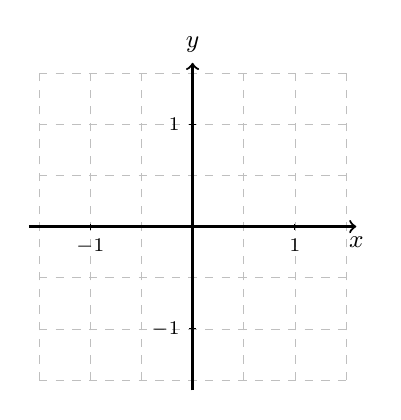
\begin{tikzpicture}[scale=1.3]
                                                                        % Hintergrund-Gitter
                                                                        \draw[step=0.5cm,gray!50,very thin,dashed] (-1.5,-1.5) grid (1.5,1.5);

                                                                        % Achsen
                                                                        \draw[->,thick] (-1.6,0) -- (1.6,0) node[below] {\small $x$};
                                                                        \draw[->,thick] (0,-1.6) -- (0,1.6) node[above] {\small $y$};

                                                                        % Achsenbeschriftungen
                                                                        \foreach \x in {-1,1} {
                                                                                \draw (\x,0.03) -- (\x,-0.03) node[below] {\scriptsize $\x$};
                                                                            }
                                                                        \foreach \y in {-1,1} {
                                                                                \draw (0.03,\y) -- (-0.03,\y) node[left] {\scriptsize $\y$};
                                                                            }
                                                                    \end{tikzpicture} $f(x)=x^3,\ g(x)=x^5$ & 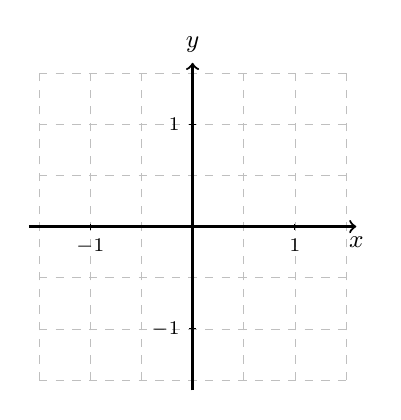
\begin{tikzpicture}[scale=1.3]
                                                                                                                  % Hintergrund-Gitter
                                                                                                                  \draw[step=0.5cm,gray!50,very thin,dashed] (-1.5,-1.5) grid (1.5,1.5);

                                                                                                                  % Achsen
                                                                                                                  \draw[->,thick] (-1.6,0) -- (1.6,0) node[below] {\small $x$};
                                                                                                                  \draw[->,thick] (0,-1.6) -- (0,1.6) node[above] {\small $y$};

                                                                                                                  % Achsenbeschriftungen
                                                                                                                  \foreach \x in {-1,1} {
                                                                                                                          \draw (\x,0.03) -- (\x,-0.03) node[below] {\scriptsize $\x$};
                                                                                                                      }
                                                                                                                  \foreach \y in {-1,1} {
                                                                                                                          \draw (0.03,\y) -- (-0.03,\y) node[left] {\scriptsize $\y$};
                                                                                                                      }
                                                                                                              \end{tikzpicture} $f(x)=x^{-2},\ g(x)=x^{-4}$ & 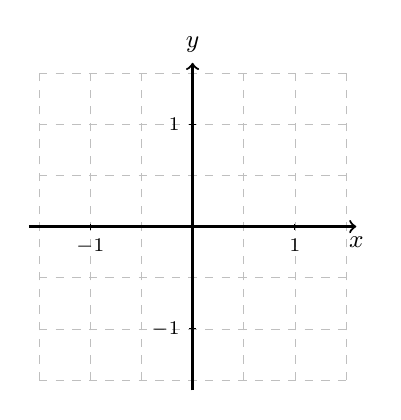
\begin{tikzpicture}[scale=1.3]
                                                                                                                                                                  % Hintergrund-Gitter
                                                                                                                                                                  \draw[step=0.5cm,gray!50,very thin,dashed] (-1.5,-1.5) grid (1.5,1.5);

                                                                                                                                                                  % Achsen
                                                                                                                                                                  \draw[->,thick] (-1.6,0) -- (1.6,0) node[below] {\small $x$};
                                                                                                                                                                  \draw[->,thick] (0,-1.6) -- (0,1.6) node[above] {\small $y$};

                                                                                                                                                                  % Achsenbeschriftungen
                                                                                                                                                                  \foreach \x in {-1,1} {
                                                                                                                                                                          \draw (\x,0.03) -- (\x,-0.03) node[below] {\scriptsize $\x$};
                                                                                                                                                                      }
                                                                                                                                                                  \foreach \y in {-1,1} {
                                                                                                                                                                          \draw (0.03,\y) -- (-0.03,\y) node[left] {\scriptsize $\y$};
                                                                                                                                                                      }
                                                                                                                                                              \end{tikzpicture} $f(x)=x^{-3},\ g(x)=x^{-5}$                                                                                                                       \\
        \hline
        Def-Bereich $\mathbb{D}$              & $\mathbb{R}$                                                                                                                 &                                                                        &                                                                        &                          \\
        \hline
        Wertemenge $\mathbb{W}$               & $\mathbb{R}^+_0$                                                                                                             &                                                                        &                                                                        &                          \\
        \hline
        Nullstellen                           & $x=0$                                                                                                                        &                                                                        &                                                                        &                          \\
        \hline
        Symmetrie                             & Gerade Funktion

        (=Achsensymmetrisch zur y-Achse)      &                                                                                                                              &                                                                        &                                                                                                   \\
        \hline
        Nachweis der Symmetrie                & $f(-x) =(-x)^n$

        $=(-1)^n\cdot x^n$

        $\stackrel{n \text{ gerade}}{=} 1\cdot x^n$

        $=f(x)$                               &                                                                                                                              &                                                                        &                                                                                                   \\
        \hline
        Quadranten                            & Verläuft im 1. und 2. Quadrant                                                                                               &                                                                        &                                                                        &                          \\
        \hline
        Monotonie                             & Monoton fallend auf $\mathbb{R}^-_0$ und monoton steigend auf $\mathbb{R}^+_0$                                               &                                                                        &                                                                        &                          \\ \hline
    \end{tabular}
\end{landscape}

\begin{example}
    Für welche $x$ gilt $x^{-3}>-125$?
    \kariert{20}
\end{example}

\subsection{Übungen (ohne Geogebra)}
Verwenden Sie die Erkenntnisse aus der letzten Aufgabe, um folgende Fragen zu beantworten.

\begin{enumerate}
    \item Die Funktionen \( f \) und \( g \) sind beides Potenzfunktionen mit unterschiedlichen, positiven, geraden Exponenten. Welche Schnittpunkte besitzen die Graphen?

    \item Die Funktion \( f \) ist eine Potenzfunktion mit positivem, ungeradem Exponenten, \( g \) eine mit negativem, geradem Exponenten. Welche Schnittpunkte besitzen die Graphen?

    \item Für welche \( x \) gilt (Tipp: fertigen Sie eine grobe Skizze des beteiligten Graphen):
          \begin{enumerate}
              \item \( x^3 < 64 \)
              \item \( x^{-2} < 25 \)
              \item \( x^6 < 64 \)
              \item \( x^{-3} < 27 \)
          \end{enumerate}

    \item Skizzieren Sie die Graphen der entsprechenden Funktionen und lösen Sie damit die Ungleichung:
          \begin{enumerate}
              \item \( x^2 \geq x^4 \)
              \item \( x^3 \geq x^5 \)
              \item \( x^{-2} \geq x^{-4} \)
              \item \( x^{-4} \geq x^3 \)
              \item \( x^{-3} \geq x^5 \)
          \end{enumerate}
\end{enumerate}
\subsubsection{Lösungen}
\begin{enumerate}
    \item \( (-1|1),\ (0|0)\ \text{und}\ (1|1) \)
    \item Nur \( (1|1) \)
    \item
          \begin{enumerate}
              \item \( \, ]{-\infty}, 4[ \)
              \item \( \, ]{-\infty}, -\tfrac{1}{5}[ \, \cup \, ]\tfrac{1}{5}, \infty[ \)
              \item \( \, ]{-2}, 2[ \)
              \item \( \, \mathbb{R}^- \cup \, ]\tfrac{1}{3}, \infty[ \)
          \end{enumerate}
    \item
          \begin{enumerate}
              \item \( [-1,1] \)
              \item \( \, ]{-\infty}, -1] \cup [0,1] \)
              \item \( \, ]{-\infty}, -1] \cup [1, \infty[ \)
              \item \( \, ]{-\infty}, 1] \setminus \{0\} \)
              \item \( \, ]{-\infty}, -1] \cup ]0,1] \)
          \end{enumerate}
\end{enumerate}
\newpage
\subsection{Funktionsgraphen verschieben und spiegeln}
Sie haben im vorherigen Kapitel die Potenzfunktionen $y=x^n,\ n\in \mathbb{Z}$ kennengelernt. Je nachdem, ob $n$ gerade, ungerade, negativ oder positiv ist, gibt es vier fundamental unterschiedliche Graphen.

Im Folgenden werden Sie anhand der Funktion $f:y=x^3$ herausfinden, welchen Effekt verschiedene Manipulationen der Funktionsgleichung auf den Graphen haben.

\subsubsection{Einführungsaufgabe}
Lösen Sie die folgende Aufgabe mit Geogebra. Skizzieren Sie jeweils den Graphen der angegebenen Funktion ins Koordinatensystem.
\smallskip
\begin{enumerate}
    \item \mbox{ $y=x^3+2$}

          \begin{minipage}{0.35\textwidth}
              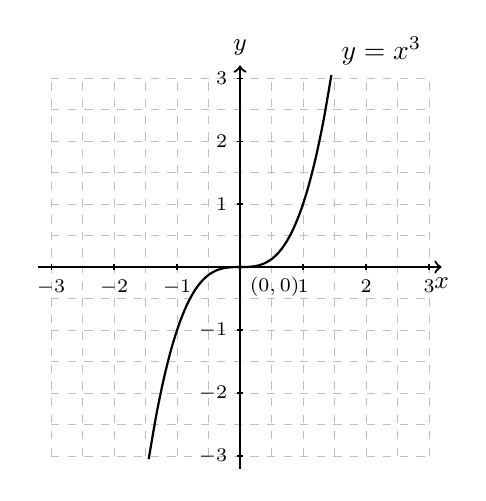
\begin{tikzpicture}[scale=0.8]
                  % Hintergrund-Gitter
                  \draw[step=0.5cm,gray!50,very thin,dashed] (-3,-3) grid (3,3);

                  % Achsen
                  \draw[->,thick] (-3.2,0) -- (3.2,0) node[below] {\small $x$};
                  \draw[->,thick] (0,-3.2) -- (0,3.2) node[above] {\small $y$};

                  % Funktionen
                  \draw[domain=-1.45:1.45,smooth,variable=\x,thick] plot ({\x},{\x*\x*\x}) node[above right] {$y=x^3$};

                  % Punkt
                  \filldraw (0,0) circle (0.8pt) node[below right] {\scriptsize $(0,0)$};

                  % Achsenbeschriftungen
                  \foreach \x in {-3,-2,-1,1,2,3} {
                          \draw (\x,0.05) -- (\x,-0.05) node[below] {\scriptsize $\x$};
                      }
                  \foreach \y in {-3,-2,-1,1,2,3} {
                          \draw (0.05,\y) -- (-0.05,\y) node[left] {\scriptsize $\y$};
                      }
              \end{tikzpicture}
          \end{minipage}
          \begin{minipage}[b]{0.7\textwidth}
              \begin{description}
                  \item[Änderung:] Addition einer Konstanten zum Funktionsterm
                  \item[Effekt auf den Graphen:]
                  \item[Erklärung für den Effekt:]
              \end{description}
          \end{minipage}
    \item \mbox{ $y=(x-1)^3$}
    
          \begin{minipage}{0.35\textwidth}
              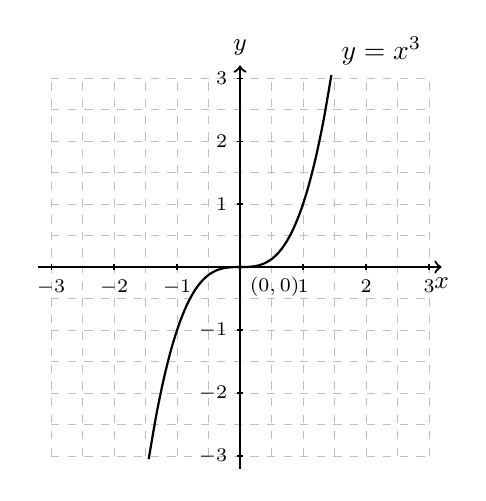
\begin{tikzpicture}[scale=0.8]
                  % Hintergrund-Gitter
                  \draw[step=0.5cm,gray!50,very thin,dashed] (-3,-3) grid (3,3);

                  % Achsen
                  \draw[->,thick] (-3.2,0) -- (3.2,0) node[below] {\small $x$};
                  \draw[->,thick] (0,-3.2) -- (0,3.2) node[above] {\small $y$};

                  % Funktionen
                  \draw[domain=-1.45:1.45,smooth,variable=\x,thick] plot ({\x},{\x*\x*\x}) node[above right] {$y=x^3$};

                  % Punkt
                  \filldraw (0,0) circle (0.8pt) node[below right] {\scriptsize $(0,0)$};

                  % Achsenbeschriftungen
                  \foreach \x in {-3,-2,-1,1,2,3} {
                          \draw (\x,0.05) -- (\x,-0.05) node[below] {\scriptsize $\x$};
                      }
                  \foreach \y in {-3,-2,-1,1,2,3} {
                          \draw (0.05,\y) -- (-0.05,\y) node[left] {\scriptsize $\y$};
                      }
              \end{tikzpicture}
          \end{minipage}
          \begin{minipage}[b]{0.7\textwidth}
              \begin{description}
                  \item[Änderung:]
                  \item[Effekt auf den Graphen:]
                  \item[Erklärung für den Effekt:]
              \end{description}
          \end{minipage}
    \item \mbox{ $y=2x^3$}

          \begin{minipage}{0.35\textwidth}
              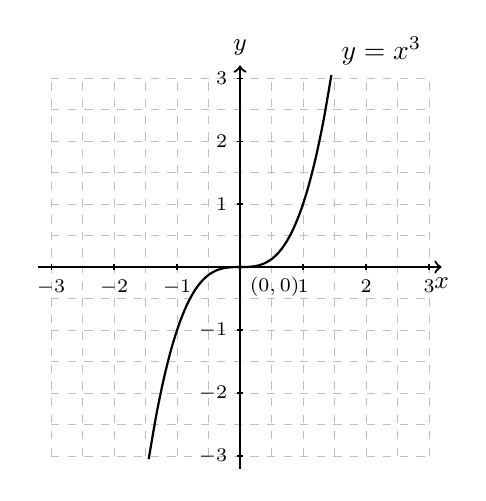
\begin{tikzpicture}[scale=0.8]
                  % Hintergrund-Gitter
                  \draw[step=0.5cm,gray!50,very thin,dashed] (-3,-3) grid (3,3);

                  % Achsen
                  \draw[->,thick] (-3.2,0) -- (3.2,0) node[below] {\small $x$};
                  \draw[->,thick] (0,-3.2) -- (0,3.2) node[above] {\small $y$};

                  % Funktionen
                  \draw[domain=-1.45:1.45,smooth,variable=\x,thick] plot ({\x},{\x*\x*\x}) node[above right] {$y=x^3$};

                  % Punkt
                  \filldraw (0,0) circle (0.8pt) node[below right] {\scriptsize $(0,0)$};

                  % Achsenbeschriftungen
                  \foreach \x in {-3,-2,-1,1,2,3} {
                          \draw (\x,0.05) -- (\x,-0.05) node[below] {\scriptsize $\x$};
                      }
                  \foreach \y in {-3,-2,-1,1,2,3} {
                          \draw (0.05,\y) -- (-0.05,\y) node[left] {\scriptsize $\y$};
                      }
              \end{tikzpicture}
          \end{minipage}
          \begin{minipage}[b]{0.7\textwidth}
              \begin{description}
                  \item[Änderung:]
                  \item[Effekt auf den Graphen:]
                  \item[Erklärung für den Effekt:]
              \end{description}
          \end{minipage}
          \newpage
    \item \mbox{ $y=\frac{1}{2}x^3$}

          \begin{minipage}{0.35\textwidth}
              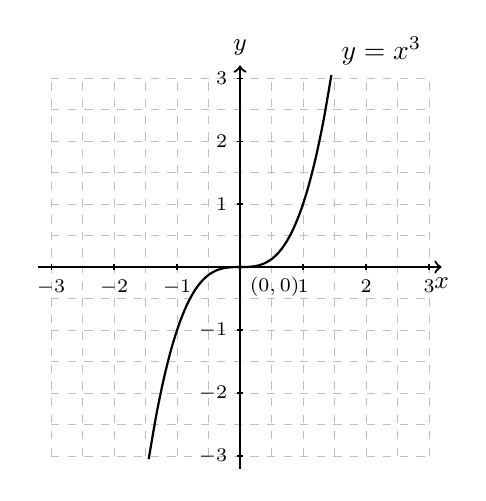
\begin{tikzpicture}[scale=0.8]
                  % Hintergrund-Gitter
                  \draw[step=0.5cm,gray!50,very thin,dashed] (-3,-3) grid (3,3);

                  % Achsen
                  \draw[->,thick] (-3.2,0) -- (3.2,0) node[below] {\small $x$};
                  \draw[->,thick] (0,-3.2) -- (0,3.2) node[above] {\small $y$};

                  % Funktionen
                  \draw[domain=-1.45:1.45,smooth,variable=\x,thick] plot ({\x},{\x*\x*\x}) node[above right] {$y=x^3$};

                  % Punkt
                  \filldraw (0,0) circle (0.8pt) node[below right] {\scriptsize $(0,0)$};

                  % Achsenbeschriftungen
                  \foreach \x in {-3,-2,-1,1,2,3} {
                          \draw (\x,0.05) -- (\x,-0.05) node[below] {\scriptsize $\x$};
                      }
                  \foreach \y in {-3,-2,-1,1,2,3} {
                          \draw (0.05,\y) -- (-0.05,\y) node[left] {\scriptsize $\y$};
                      }
              \end{tikzpicture}
          \end{minipage}
          \begin{minipage}[b]{0.7\textwidth}
              \begin{description}
                  \item[Änderung:]
                  \item[Effekt auf den Graphen:]
                  \item[Erklärung für den Effekt:]
              \end{description}
          \end{minipage}
    \item \mbox{ $y=-x^3$}

          \begin{minipage}{0.35\textwidth}
              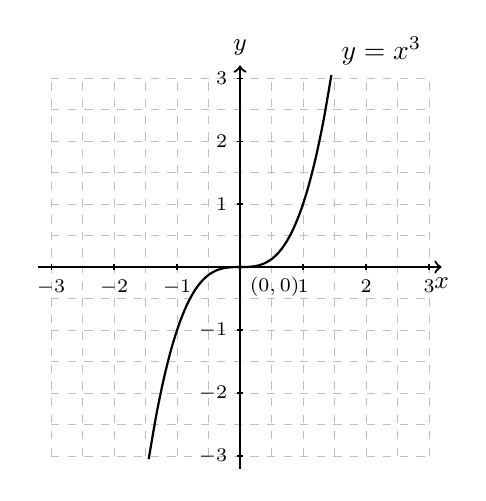
\begin{tikzpicture}[scale=0.8]
                  % Hintergrund-Gitter
                  \draw[step=0.5cm,gray!50,very thin,dashed] (-3,-3) grid (3,3);

                  % Achsen
                  \draw[->,thick] (-3.2,0) -- (3.2,0) node[below] {\small $x$};
                  \draw[->,thick] (0,-3.2) -- (0,3.2) node[above] {\small $y$};

                  % Funktionen
                  \draw[domain=-1.45:1.45,smooth,variable=\x,thick] plot ({\x},{\x*\x*\x}) node[above right] {$y=x^3$};

                  % Punkt
                  \filldraw (0,0) circle (0.8pt) node[below right] {\scriptsize $(0,0)$};

                  % Achsenbeschriftungen
                  \foreach \x in {-3,-2,-1,1,2,3} {
                          \draw (\x,0.05) -- (\x,-0.05) node[below] {\scriptsize $\x$};
                      }
                  \foreach \y in {-3,-2,-1,1,2,3} {
                          \draw (0.05,\y) -- (-0.05,\y) node[left] {\scriptsize $\y$};
                      }
              \end{tikzpicture}
          \end{minipage}
          \begin{minipage}[b]{0.7\textwidth}
              \begin{description}
                  \item[Änderung:]
                  \item[Effekt auf den Graphen:]
                  \item[Erklärung für den Effekt:]
              \end{description}
          \end{minipage}
\end{enumerate}
\newpage
\subsubsection{Beispiele}
\begin{example}
    Zeichnen Sie den Graphen von $y=(x+2)^{-1} +1$
    \kariert{21}
\end{example}
\begin{example}
    Zeichnen Sie den Graphen von $y=3(x-2)^{4} - 6$
    \kariert{21}
\end{example}
\newpage
\begin{example}
    Geben Sie die Funktionsgleichung des um 5 Einheiten nach rechts und eine Einheit nach unten verschobenen Graphen von $y=\frac{1}{x^7}$ an.
    \kariert{5}
\end{example}

\begin{example}
    Geben Sie die Funktionsgleichung des an der y-Achse gespiegelten Graphen von $y=(x+3)^2+1$ an.
    \kariert{10}
\end{example}
\subsubsection{Übungen}
Algebra 9/10, S.160 folgende: 141, 144, 145, 146, 148, 152
